\section{Evaluation}
\label{eval}

We have used the YFCC100M dataset to evaluate different aspects of our system.
We use the images in the dataset and its associated metadata to implement
an image-search engine based on properties associated with those images.
This is a very common use-case we have encountered when building
applications such as smart-retail, sports applications, and video summarization.
For these type of applications, the starting point is usually
a large set of data that must be curated
before proceeding with the data processing (such as neural network training).
In order to evaluate the different aspects of the performance on the
image search, we have built different baselines following the methodology
used in the industry, and following what we have done in the past
in order to build an image search engine, which we describe in Section \ref{images}.
% We have also included performance evaluation on the Video and Feature Vectors
% functionality in the appendix for further reference, together with a
% description of the key aspects of those functionalities.

\begin{figure*}
\centering
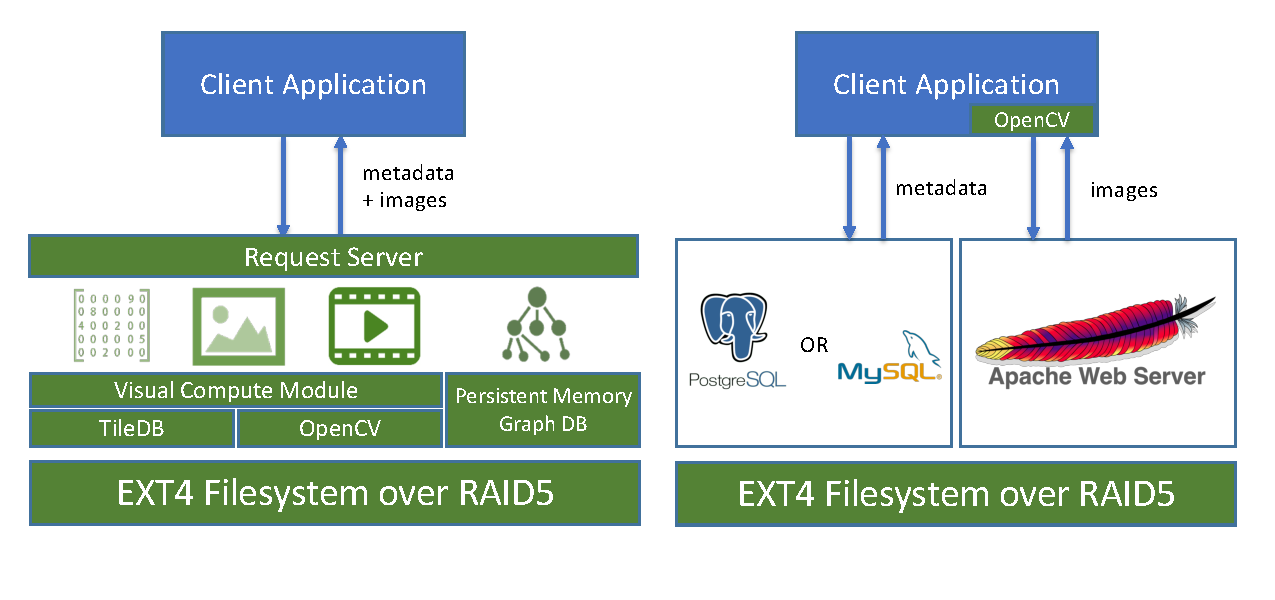
\includegraphics[width=\textwidth]{figures/comparison_system}
\caption{Comparison Systems: Logical view of the interaction between the client application with VDMS (left) and the baseline systems based on Apache Web Server and PostgreSQL (middle), or MySQL (right). The image repository is shared.}
\label{fig:systems}
\end{figure*}

\subsection{YFCC100M Dataset}
\label{dataset}

The Yahoo! Flickr Creative Commons 100m (YFCC100M) dataset is a large
collection of 100 million public Flickr media objects created to provide free,
shareable multimedia data for research.
This dataset contains approximately 99.2 million images and 0.8 million videos
with metadata characterized by 25 fields such as the unique identifier, userid,
date the media was taken/uploaded, location in longitude/latitude coordinates,
device type the media was captured, URL to download the media object,
and the Creative Commons license type information.
The YFCC100M dataset also contains \textit{autotags}
provided as a set of comma-separated concepts such as people, scenery, objects,
and animals from 1,570 trained machine learning classifiers ~\cite{Thomee_2016}.
Together with each \textit{autotags}, there is a probability associated with
each tag to indicate certainty of the classification.
This is, an image can have the \textit{autotags} "people", "person", "party",
"outdoor", and each \textit{autotag} assigned will be accompanied by a
probability of that \textit{autotags} being present in that image/frame.
% We have also used feature vectors generated for every image and first frame
% of every video \cite{features} to implement a similarity search.
Given that there is no standard benchmark oriented towards visual data queries,
we have built a series of queries to filter this dataset that is modeled after
our internal use cases for many of the mentioned applications we have worked
with.

\subsection{Experimental Setup}
\label{setup}

Given that there are no other open-source systems that provide similar
functionality and interfaces as VDMS (i.e., transactionally dealing with images
and metadata behind a single interface), we have implemented two equivalent
visual data management system as baselines,
design specifically for the image search use case,
and comprised of a combination of widely available, off-the-shelf components.
The first baseline uses MySQL Server 5.7 (for storing metadata),
Apache Web Server 2.4.18 (as interface for image access), and
OpenCV 3.3 (to provide pre-processing operations on images).
We chose Apache Web Server to work as a file server (serving the image files),
because it provides the lowest possible overhead
(when compared to other object store system), at the expenses of providing less
functionality (authentication, data integrity checking, etc).
The other baseline system replaces the MySQL Server 5.7 with a
most advanced open-source relational database, PostgreSQL 9.5 \cite{postgresql}.
We decided to use relational databases in the baseline systems instead of
non-relational databases because of their maturity, and also because it is
the most common tools used for storing and querying metadata
~\cite{Jatana2012, li_2019}:

\begin{itemize}
    \item Relational databases support atomicity, consistency, isolation,
    and durability (ACID) while non-relational may compromise some ACID properties.
    \item The YFCC100m data is clearly structured, and can be modeled with relatively ease with a relational database.
    \item We need to efficiently collate and return metadata records,
    and SQL engines are very mature and optimized for that task.
\end{itemize}

The baseline implementations only partially replicate the functionalities
that VDMS offers when it comes to image and metadata handling, and it was
built for the purpose of an ad-hoc image search implementation.
The baseline implementations are based upon internal tools used for ML-based
pipelines for visual data, which is common practice
in the industry \cite{haystack, tao}.
We have implemented a set of client-side applications that take care
of retrieving the components from the different systems, and applies
pre-processing operations when needed.

For all our experiments, we use two servers with Ubuntu 20.04,
one hosting a VDMS server and another hosting the baseline implementations.
Both servers have a dual-socket Intel\textsuperscript{\textregistered}
Xeon\textsuperscript{\textregistered} Platinum 8180 CPU @ 2.50GHz (Skylake),
each CPU with 28 physical cores with hyper-threading enabled,
for a total of 112 logical cores per server.
The server hosting MySQL and PostgreSQL has 256GB of DDR4 DRAM,
while the server hosting VDMS has 194GB of DDR4 DRAM.
We decided to run the VDMS server in the machine with less DRAM to make
sure MySQL and PostgreSQL had no disadvantage. Previous evaluation
indicated smaller footprint in the case of VDMS when
compared to similar baselines based on MySQL.
To build both MySQL and PostgreSQL on the same machine,
we stored each database on separate SSD drives.
Other than the difference in DRAM space and storage needed for two baselines,
the machines are identical.
The client application running the queries and measuring round-trip time
is connected to the server through a 1GB wired link through
a 10GB back-plane switch, same as both servers.
The client application was implemented using Python 3 for both VDMS and the baselines.
Figure~\ref{fig:systems} shows a logical view of the difference between the
interaction of the client application (retrieves metadata and
images) with VDMS (left), the PostgreSQL baseline (middle), and the MySQL baseline (right).

It is worth noting that the images are stored in a shared repository
(ext4 filesystem on a RAID 5 configuration of 16TB) that both
Apache WebServer and VDMS have direct access.
In the case of videos, only the first frame is used for the image search.
% More information and evaluation on video-specific functionalities can be found
% in the appendix of this work.
In the case of the baselines, metadata is
stored in MySQL and PostgreSQL using an attached SSD disk.
Even if VDMS has native support for Optane Persistent Memory,
we do not use it in this experiment because of fairness of
comparison with respect to MySQL and PostgreSQL, which were not designed for
Persistent Memory type of storage.
The benefits of Persistent Memory for metadata and a full evaluation of
the PMGD subsystem is material for another paper,
and outside the scope of this evaluation.
For this experiment, in the case of VDMS we simply use a similar
attached SSD disk to store metadata.
Even if PMGD, the graph database used by VDMS, is designed for persistent memory,
it can deliver good performance when using SSDs directly.

For the metadata, we built VDMS, MySQL, and PostgreSQL databases using
the YFCC100M dataset with incremental database sizes to study the effects at scale.
For simplicity, we named the database based on the approximate number of images
it contains, as follows: 1M, 5M, 10M, 50M, 100M.
The baseline systems have comparable number of elements.
The exact number of images/elements in each database are shown in
Table \ref{table:vdmsnodes} and \ref{table:mysqltables}.
The differences can be attributed to minor failures in data
preparation/loading because of incomplete/inconsistent formatting,
which is common in large datasets \cite{failures}.
In our set up, that difference is very small: less than 0.253\% in terms of
number of elements (images and/or metadata information).

\subsubsection{Data Representation}
We detail the data representation for each of the systems we implemented:

\textbf{VDMS:}
For each database size, we created an instance of VDMS using the image/video metadata,
the machine-generated \textit{autotags} associated with
each image/video identifier, and the list of 1,570 \textit{autotags}.
Internally, that information is represented as a graph,
where we have one node for each image, one node for each tag
(always 1,570 tags), and a connection between each image and its respective tag(s).
For instance, if an image has four \textit{autotags} assigned,
there will be four connections between that image and
the different nodes for those \textit{autotags}.
The probability the \textit{autotag} is present in an image
is expressed as a property in the \textit{connection} between the two nodes.
Figure~\ref{fig:graph_representation} shows an example on two images,
two \textit{autotags}, and the \textit{connections} between
those \textit{autotags} and the images.
Image id 23143252 has two \textit{autotags} assigned:
\textit{Alligator} with probability 0.285, and \textit{Lake} with probability 0.872.
Image id 86756231, on the other hand, has a single \textit{autotags} assigned:
\textit{Alligator} with probability 0.894.
On average there are 8 tags assigned to each image so
there will be around 8 times more connections than images, as shown
in Table~\ref{table:vdmsnodes}.
Also, each image node will contain multiple properties associated
with it (some of which are listed in Section \ref{dataset}).
% Using the Python Client Module, we insert 1,570 nodes for the \textit{autotags},
% and then insert nodes for the YFCC media objects (images or videos)
% with the associated metadata (as properties of the image/video).
% Then, for each image, we add a \textit{connection} between the image node
% and the \textit{autotag} node. The probability of that \textit{autotag}
% being present in that image is stored as a property in that \textit{connection}.
The number of nodes (representing images and \textit{autotags})
are dependent on the database size and the \textit{connections} are responsible for
90\% of the elements in each database instance,
as shown in Table~\ref{table:vdmsnodes}.
It is also important to note that we create indexes for the image identifier,
\textit{autotags} properties, and longitude/latitude coordinates
to enable faster retrieval.

\begin{figure}[ht]
\centering
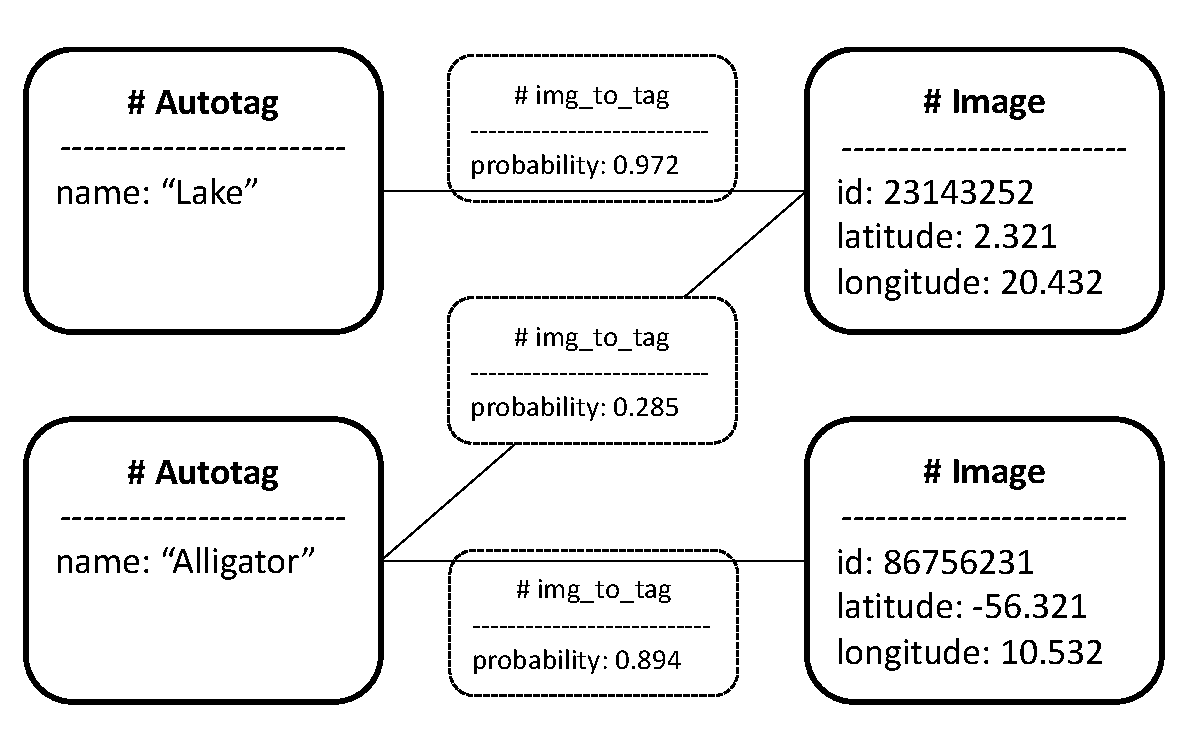
\includegraphics[width=\columnwidth]{figures/graph_representation}
\caption{VDMS Data Representation Using a Property Graph:
Example on two images and 2 \textit{autotags} with
their respective probabilities expressed in the \textit{connection}.
Image id 23143252 has two \textit{autotags} assigned:
\textit{Alligator} with probability 0.285, and \textit{Lake} with probability 0.872.
Similarly, Image id 86756231 has a single \textit{autotags} assigned:
\textit{Alligator} with probability 0.894.}
\label{fig:graph_representation}
\end{figure}

\begin{table}[ht]
\caption{VDMS Database - Number of Elements}
\centering
\begin{tabular}{c c c c}
\hline\hline
DB Name & \# Images & \# Connections & \# TagList\\
\hline
% 100k & 100,000     & 848,432      & 1,570\\
% 500k & 500,000     & 4,249,500    & 1,570\\
1M   & 1,000,000   & 8,503,045    & 1,570\\
5M   & 5,000,000   & 42,505,478   & 1,570\\
10M  & 10,000,000  & 85,040,404   & 1,570\\
50M  & 50,000,000  & 425,162,070  & 1,570\\
100M & 99,205,984  & 895,572,430  & 1,570\\
\hline
\end{tabular}
\label{table:vdmsnodes}
\end{table}

\textbf{MySQL-Based System (\textit{mysql}):}
Each MySQL database is created in a similar manner as VDMS
but the data is represented as three tables, following the relational model:
1) \textit{images} table: contains one row per image,
and a column for each property
associated with the images (some of which are listed in Section \ref{dataset});
2) \textit{taglist} table: contains one row per autotag element
(always 1,570 rows);
3) \textit{autotags} table: contains one row per autotag
assigned to an image. Each row contains a foreign key to the
image, a foreign key to the tag, and
the probability assigned to that tag belonging to that image.
Given that there are 8 autotags, on average, per image, the \textit{autotags}
table has around 8 times the number of rows present in the
\textit{metadata} table, as can be seen in Table~\ref{table:mysqltables}.
Using a Python client and simple queries, the \textit{taglist}
table is read from the list of tags with an auto-incremented
\textit{tagid} as a primary key, and the metadata table
is read from the YFCC100M metadata using the identifier as a primary key.
The \textit{autotags} table contains the generated autotags and
probabilities for entries of the \textit{images} table.
To generate the table, we split the \textit{autotags} data for each database
by the image identifier and autotag into new files.
The new files are read into the \textit{autotags} table with the image
identifier and \textit{tagid} as foreign keys.

In an attempt to have the best MySQL configuration possible for this use case,
we explore several parameters to increase the performance
of both loading the data, as well as executing the queries.
In particular, MySQL optimizes threads and transactions out-of-box,
but it cannot handle the entire YFCC100M dataset without configuring
specific parameters.
When creating large databases, a data lock may occur to protect the
data from concurrent updates~\cite{mysql_blog}.
To avoid this mechanism, we increased the buffer pool size to
increase the amount of memory allocated to internal data structures.
It is recommended to set the buffer pool size to 60-80\% of the physical
memory size ~\cite{mysql,mysql_blog}.
However, the time to build a database increased.
We later changed  the buffer pool size to be 16x the default value,
where we saw the best performance.

By default, MySQL uses the available operating system threads to
execute \textit{n} requests in parallel where \textit{n} is
the number of background read/write I/O threads.
Setting the respective parameters in the MySQL configuration file can limit the
number of concurrent threads and the number of background threads.
When a limit is set on the number of threads, and no threads are available,
requests will go into a FIFO queue until threads are available to execute
the request ~\cite{mysql,mysql_blog}.
We ran a few experiments investigating the effects of setting a limitation on the
number of concurrent and background threads.
We concluded that the default settings perform better for large databases instead of
setting a limit.
Therefore, we let MySQL automatically handle the concurrency.

\textbf{PostgreSQL-Based System (\textit{postgresql}):}
Each PostgreSQL database is created in the exact same manner as MySQL
where data is represented as three tables:
\textit{images}, \textit{taglist}, and \textit{autotags}.
PostgreSQL works well out-of-box and optimizations were not necessary,
as in MySQL, to load or execute queries.
When executing queries for larger databases,
it is pertinent to have enough disk space for both
the database and tablespace.
The tablespace is associated with a database and stores the temporary files
created within the database object ~\cite{postgresql}.
When processing the larger databases, additional
storage may be needed for the tablespace or a diskfull error may occur.
To avoid this, we allocated a separate SSD disk specifically
for the tablespace of all databases.
This was required, specially for 100M database, in order to make the queries
complete execution without failures, and represented a big disadvantage
in terms of the disk space footprint during query execution.

By default, PostgreSQL can manage concurrent access to data well using
Multiversion Concurrency Control (MVCC) and a Serializable Snapshot Isolation
(SSI) level of transaction isolation.
MVCC provides better performance by using SSI to guarantee querying data never
blocks writing data, and vice versa ~\cite{postgresql}.
The PostgreSQL configuration file initially limits the maximum
number of concurrent connections to the database server to 100.
We increased this limit to 200 to complete the concurrency analysis
in Section \ref{concurrency_analysis}.

In the case of VDMS, we did not attempt to tune any
parameter to avoid unfairness in the comparison against the baselines.
Unlike the baselines, VDMS can handle the entire YFCC100m dataset
using the default parameters provided by the implementation.

\subsubsection{Indexes:}
For all systems, we created indexes over the
properties we used for search, such as name of
\textit{autotag}, and geo-location values.
Building indexes for the right properties and objects
is basic operation that would be present in any real-world deployment,
and measuring performance without them would lead to useless analysis in our
real-world applications and use cases.

\begin{table}[ht]
\caption{MySQL and PostgreSQL Databases - Number of Rows in each Table}
\centering
\begin{tabular}{c c c c}
\hline\hline
 & \multicolumn{3}{c}{Table}\\
\cline{2-4}
DB Name & images & autotags & taglist\\
\hline
% 100k & 100,000    & 848,912     & 1,570\\
% 500k & 498,707    & 4,241,200   & 1,570\\
1M   & 1,000,000  & 8,508,380   & 1,570\\
5M   & 4,987,379  & 42,425,905  & 1,570\\
10M  & 10,000,000 & 85,095,265  & 1,570\\
50M  & 50,000,000 & 425,446,208 & 1,570\\
100M & 99,206,564 & 896,002,496 & 1,570\\
\hline
\end{tabular}
\label{table:mysqltables}
\end{table}

% \begin{figure}[ht]
% \centering
% 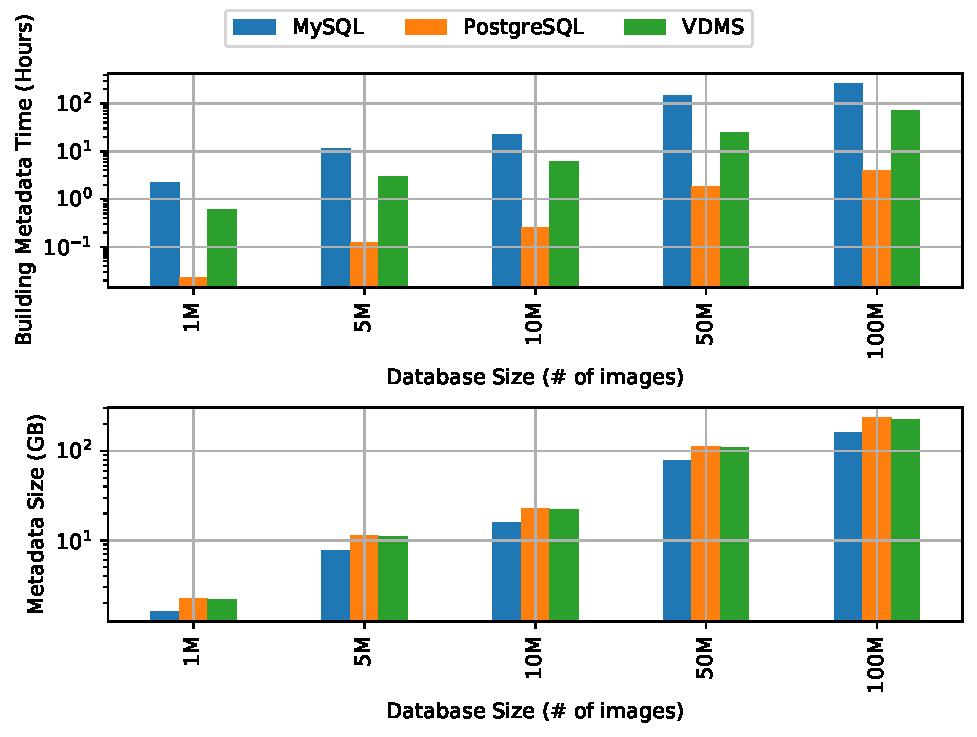
\includegraphics[width=\columnwidth]{figures/all_build_times_plot}
% \caption{Time to build and size (in GB) of MySQL, PostgreSQL, and VDMS databases.}
% \label{fig:db_time_size}
% \end{figure}

\begin{figure}[ht]
\centering
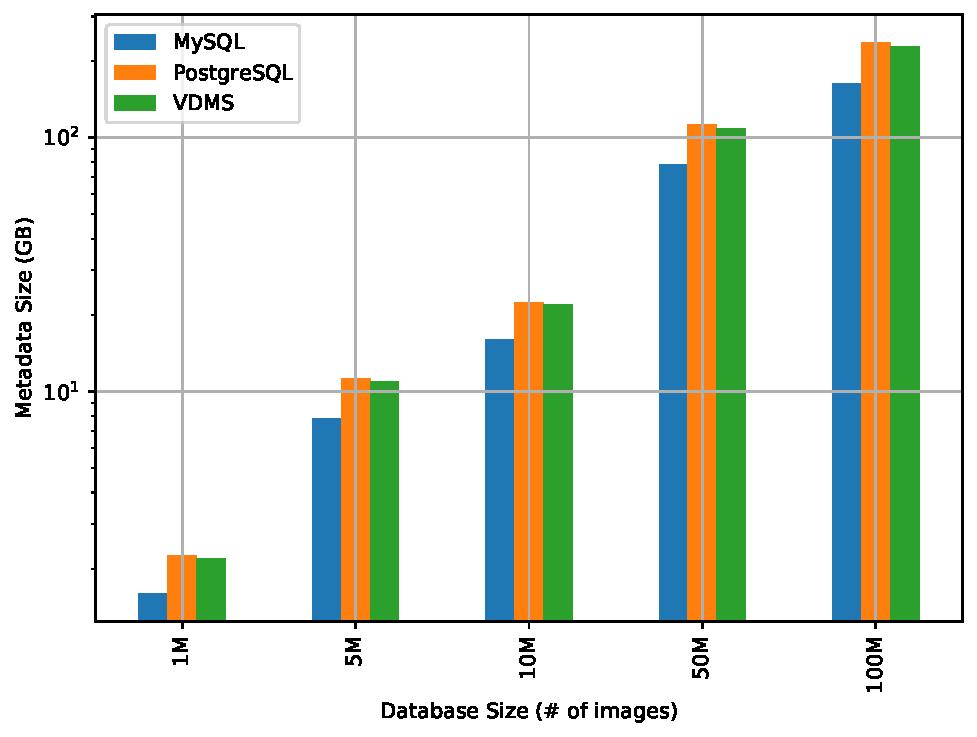
\includegraphics[width=0.8\columnwidth]{figures/all_build_sizes_plot}
\caption{Data footprint (in GB) of MySQL, PostgreSQL, and VDMS databases.}
\label{fig:db_sizes}
\end{figure}

\subsubsection{Database Storage Footprint}

The Graph Database used by VDMS (PMGD) was designed for performance,
especially in environments where persistent memory is present.
This design decision comes as a trade-off for storage footprint, which is
noticeable in other PMGD evaluation we have run in the past.
Because PMGD was not optimized for low storage footprint, authors feared that
any improvement would come at the expenses of a significant increase on
disk occupancy.
We measured metadata disk footprint for that reason, and show the results
in Figure~\ref{fig:db_sizes}.
PostgreSQL and VDMS require comparable amount of storage for metadata which
is more than required by MySQL, shown in Figure~\ref{fig:db_sizes}.
In the case of VDMS, this is space used to store information about
each node/connection.
VDMS required 37-41\% more storage than MySQL for storing the same amount
of metadata. On the other hand, PostgreSQL required 1-4\% more storage than VDMS.
The storage footprint may become a factor if storage is a limitation, but
it should also be noted that metadata accounts for less than 2\% of the
overall database size even if we have a 41\% increase in metadata size.
For example, the largest database (both metadata and images) we built
(100M) has around 230GB of metadata and 12TB of images.
In systems where persistent memory is a scarce resource,
the increased storage footprint of PMGD may represent a challenge.
On the other hand, persistent memory is expected to be available
in the order of TBs per server, which should fit the
metadata of intensive use-cases\cite{IntelXPoint15}.

%=========================================

\subsection{Images Search}
\label{images}

In order to evaluate VDMS and the baseline systems for our use-case queries,
we implemented 6 queries that filter and retrieve a specific set of images.
We chose these queries because they are the same that we use when filtering a
cohort of images to be retrieved and processed from a large corpus of data.
As we mentioned before, we took this approach mainly because we wanted to
replicate systems we have built internally for our use cases,
and also because of the lack of standard
benchmarks that are oriented towards visual data retrieval.

The implementation of this evaluation, as well as all the queries, are available
open-source for reproducibility
\footnote{https://github.com/luisremis/visual\_storm/tree/master/yfcc100m},
together with all the results of our evaluation
\footnote{https://github.com/luisremis/visual\_storm/tree/master/yfcc100m/python/eval/results}.

We use the metadata associated with the images to filter the images.
We use the \textit{autotags} (as they contain information about the content
of the image), and geo-location information (latitude/longitude)
of the images for search and filtering.
Note that, even if we use geo-location for our study, any other property
assigned to the images can be used to refine the search
in both VDMS and baseline implementations.
On top of that, and for our use cases, we would like to extract more information
about the content of the image through the use of ML,
such as Convolutional Neural Networks~\cite{cnn}.
For this, we resize the images to 224x224, which is the input layer size for
popular variations of neural networks for object detection on images~\cite{resnet}.
We used both ResNet and Yolov3 for object detection, both of which
have the requirement of a downsized, lower resolution image as input.

To evaluate the access to metadata and images,
we use the following queries, based on our internal use cases:

\begin{itemize}
\item \textit{q1} - {\bf {\em 1tag\_resize}}: Retrieve images with one specific autotag and resize to 224x224.

\item \textit{q2} - {\bf {\em 1tag\_geo\_resize}}: Retrieve images with one specific autotag, in a particular geo-location, and resize to 224x224,.

\item \textit{q3} - {\bf {\em 2tag\_resize\_and}}: Retrieve images with two specific autotags (i.e. alligator AND lake), and resize to 224x224.

\item \textit{q4} - {\bf {\em 2tag\_resize\_or}}: Retrieve images with either of two specific autotags (i.e. alligator OR lake), and resize to 224x224.

\item \textit{q5} - {\bf {\em 2tag\_geo\_resize\_and}}: Retrieve images with two specific autotags (i.e. alligator AND lake), in a particular geo-location, and resize to 224x224.

\item \textit{q6} - {\bf {\em 2tag\_geo\_resize\_or}}: Retrieve images with either of two specific autotags (i.e. alligator OR lake), in a particular geo-location, and resize to 224x224.

\end{itemize}

It is important to note that when querying for images with certain
\textit{autotags}, we also apply a filter using the probability.
For instance, we only retrieve images with an autotag \textit{alligator}
and a probability higher than 92\%.
These probabilities are both present in VDMS (in the form of a property
of the \textit{connection} between the image and that \textit{autotag}),
as well as in \textit{mysql} and \textit{postgresql} (in the form of a column in the
\textit{autotags} table that links images with tags).
In the case of VDMS, the query involves a graph traversal query that starts
from the \textit{autotag} node and ends in the images node,
following \textit{connections} between the image and that \textit{autotag}).
In the case of the baseline implementations,
the query involves JOIN operations between the 3 tables.

Also, note that the size of the result (number of images retrieved)
is linear with the size of the database. This is, if a query returns 100 images
for the 1M database, it will return around 1000 images for the 10M database.
This poses a problem when evaluating performance as the size of the database increase,
and clearly understanding the measurements.
Because of this reason, we control the number of returned images for all the
databases using the probability of the \textit{autotags}
(higher probabilities returns less images), so that the queries in
this experiment return a similar number of images for all database sizes.
In other words, as the size of the database increase, we increase the probability
threshold for the queries. We do this for both VDMS and the baselines, of course.
This way, we remove bottleneck introduced by network bandwidth that would
otherwise over-complicate the understanding of the results,
and play in disadvantage for the baseline implementations.

Image search based on metadata is very expensive in large databases.
Because of the large volume of data, the processing of the retrieved images
is performed in parallel, using multi-core and/or distributed systems.
For instance, a common implementation of an image processing pipeline
would involve the use of distributed processing frameworks
like Hadoop \cite{hadoop} or Spark \cite{spark}.
Consequently, it is key that the data management system used supports
concurrency, providing multiple workers with data in parallel.
The ability to scale with the number of simultaneous clients is key for the
applicability of visual data management systems like VDMS.
Because of this, \textit{we put emphasis on the analysis of
\textbf{concurrency and throughput}, rather than latency}.


%% ========= Concurrency Comparison Analysis

\subsubsection{Concurrency Analysis} \label{concurrency_analysis}

\begin{figure}[ht]
% WAS: begin{figure*}[ht]; textwidth
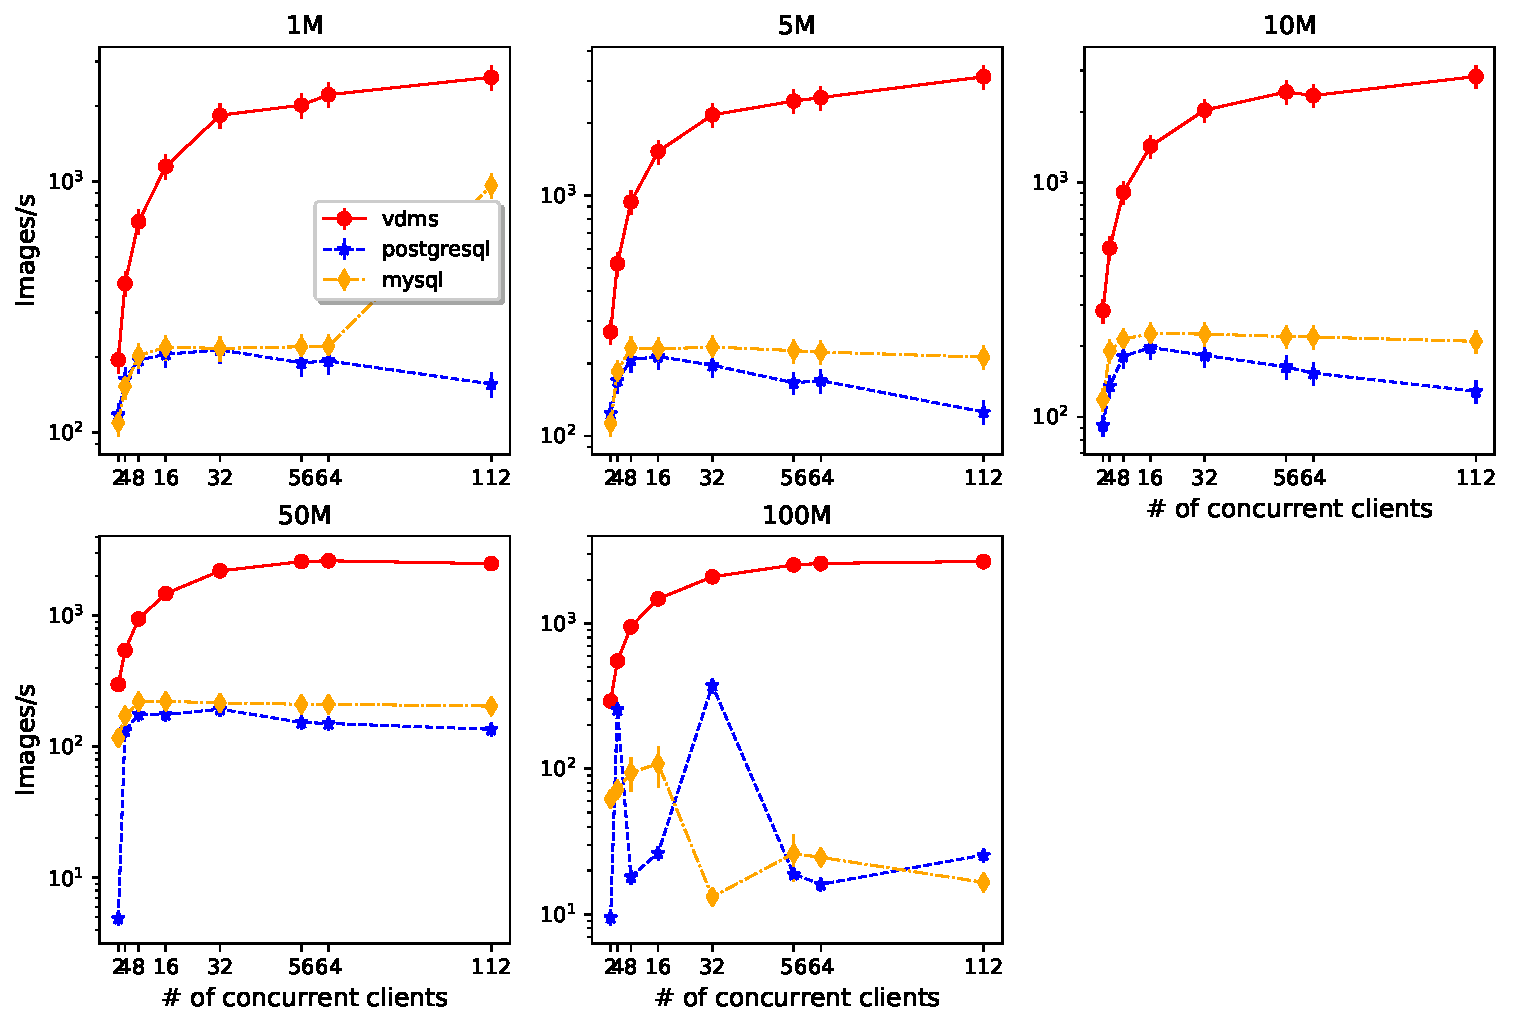
\includegraphics[width=\columnwidth]{figures/plot_conc_q_1tag_geo_resize_mosaic_results_throughput_db_size}
\caption{Concurrency Analysis on \textit{q2} (\textit{1tag\_geo\_resize}) from our use-case
described in the Experimental Setup Section.
The figures show the throughput (images per second) when retrieving
resized versions of the images, as the number of concurrent clients increases.
Hardware concurrency (number of physical cores in each system)
is 56.}
\label{fig:concurrency_comparison_q2}
\end{figure}

To analyze these results, one needs to compare the full-line (VDMS) versus the
dotted-lines (two baselines).
We start with a simple query that involves a simple
metadata filtering over 1 tag and also geo-location,
plus pre-processing operations.
Figure~\ref{fig:concurrency_comparison_q2} illustrates a concurrency analysis
for \textit{q2} (\textit{1tag\_geo\_resize}), described above,
using VDMS and the baselines.
Here we evaluate the concurrency of all systems, as the number of concurrent
clients grows (x-axis) and as the size of the databases grow.
Figure~\ref{fig:concurrency_comparison_q2} shows throughput (images per second)
when retrieving resized versions of the images, as the number of
concurrent clients increase.
The first thing to notice is that VDMS outperforms both baselines for all
databases for this query by a large margin.
For the baseline systems, in the case of 100M, the increase in the
size of data seems to have a larger impact in performance.
This result can be attributed to the increase in the complexity of the JOIN
operation as the number of rows in the tables increases.

Another thing to notice is that, as the number of concurrent clients increases,
VDMS throughput continues to increase up to 56 threads, which is
the hardware concurrency of the system.
Also, more parallelism after 56 threads does not increase the delivered throughput
for the larger databases (50M and 100M) but there is a slight improvement in the
other databases (1M, 5M, and 10M).
On the other hand, both baselines seem to deliver less aggregated
throughput after 16 threads except for the 100M case.
In this case, \textit{postgresql} has a performance spike at 32 clients
and the performance for both baselines is less stable when compared
to VDMS.
Note that most of the throughput for the baseline systems are very close to each other.
This is mostly an effect of the log-scale used, which is needed to clearly
depict the difference between VDMS and the baselines.
Here, the baselines are the full architectures described in
Figure~\ref{fig:systems} (middle and right).

All queries run a resize operation on the image,
an operation that requires decoding, resizing, and encoding the image
before sending it back to the client.
These operations are mainly compute bound, and that is the reason for
the system to stop scaling beyond the number of physical cores.
In contrast, the baseline does not scale nearly as well as VDMS,
and we see that even after increasing concurrency, the increase
in throughput is just about 2x.
When comparing the case of 56 or 64 concurrent clients,
VDMS delivers between 8x and 10X the throughput.

\begin{figure}[ht]
% WAS: begin{figure*}[ht]; textwidth
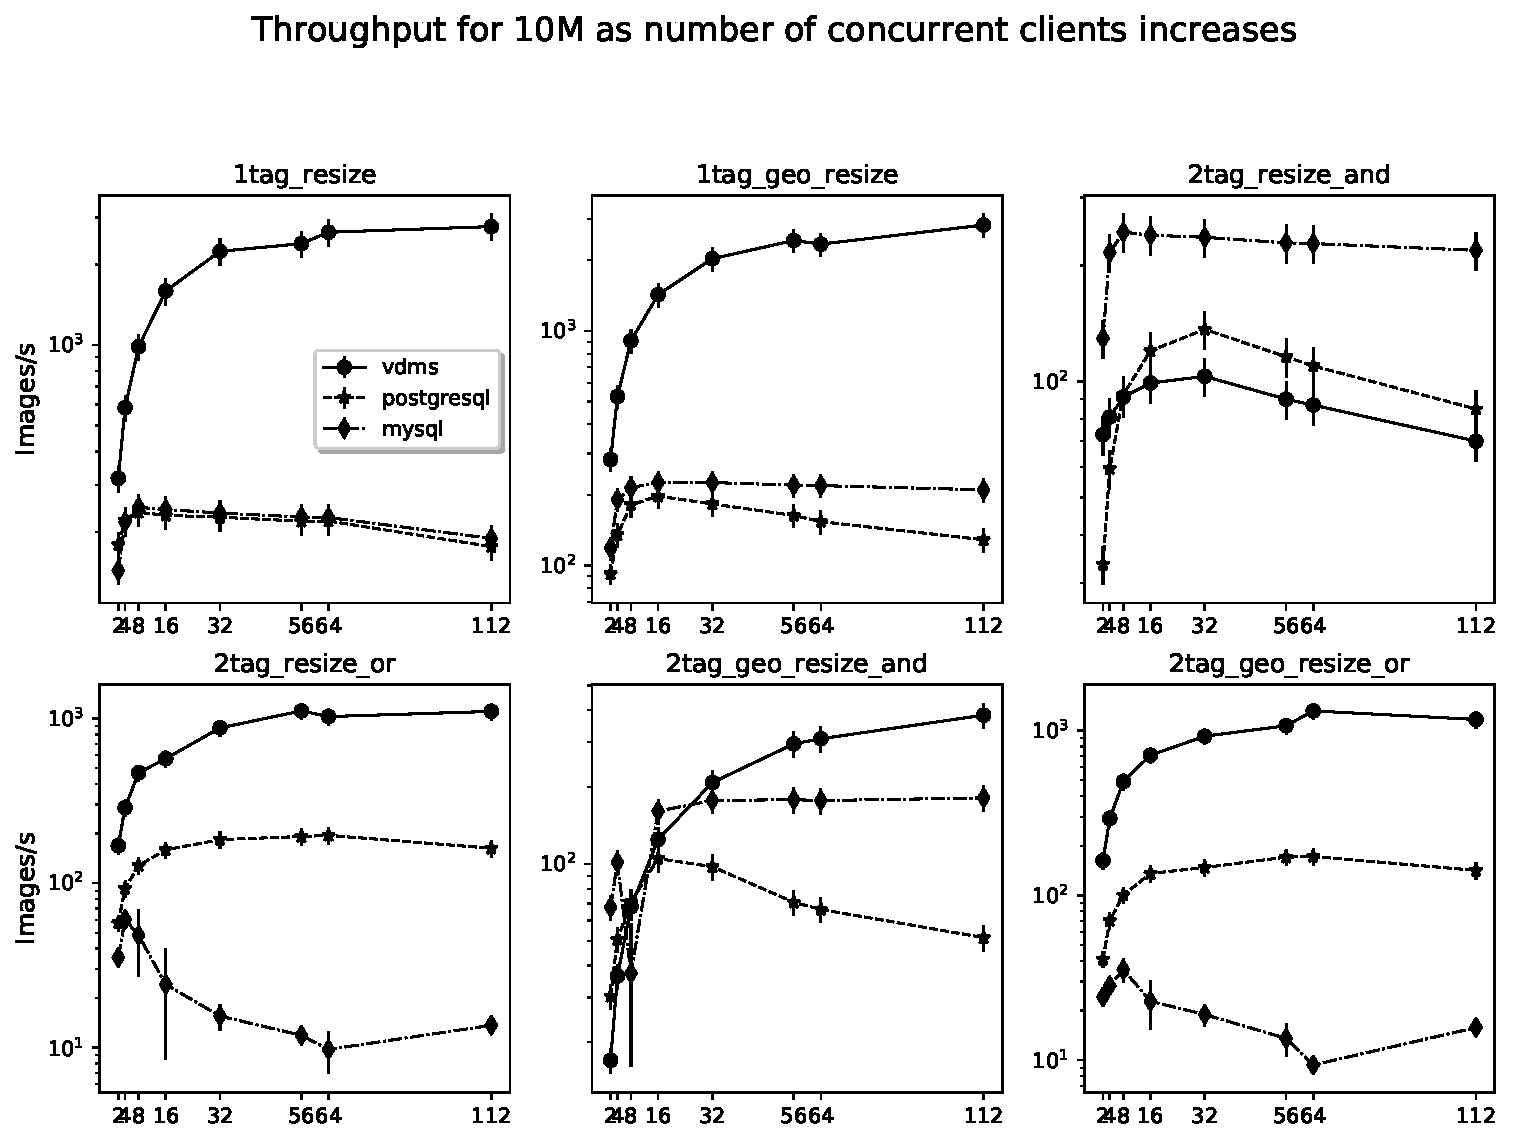
\includegraphics[width=\columnwidth]{figures/plot_conc_dbsize_10M_mosaic_results_throughput}
\caption{Concurrency Analysis for all the queries using the 10M database.
Each figure shows the throughput (images per second) when retrieving
resized versions of the images as the number of concurrent clients increases.
Hardware concurrency (number of physical cores in each system)
is 56.}
\label{fig:concurrency_comparison_10M}
\end{figure}

We continue by looking at Figure~\ref{fig:concurrency_comparison_10M}
which shows the images per second delivered by each system
for all queries using the 10M database, as the number of concurrent
clients grows (x-axis). This figure takes a closer look at the
concurrency for each of the six queries.
VDMS consistently outperforms each of the baseline
systems for queries \textit{q1}, \textit{q2}, \textit{q4},
and \textit{q6} as concurrency grows. This figure
shows a similar trend as Figure~\ref{fig:concurrency_comparison_q2}
when it comes to concurrency.  The
VDMS throughput continues to significantly increase up to 56 concurrent clients,
which is the hardware concurrency of the system, for all queries except \textit{q3}.
In this query, the throughput seems to decrease after 32 clients
and both baselines outperform VDMS after 8 concurrent clients.
Prior to 8 clients, VDMS has a slight advantage over \textit{postgresql} which has
a major performance improvement at 16 concurrent clients. On the other hand,
\textit{mysql} maintains its improvement in throughput over \textit{postgresql}
and VDMS over all concurrent clients.
In the case of \textit{q5}, the throughput of the baselines
are less aggregated than those of VDMS up to 16 concurrent clients. When it comes
to low concurrency, the baselines do as good and even better than VDMS with 2 or
4 concurrent clients.
At 16 concurrent client, the performance of the \textit{mysql} baseline
begin to stabilize while the throughput of \textit{postgresql} begins to degrade.
However, as concurrency increases beyond 16 concurrent clients, the difference
in throughput becomes clear, with VDMS reaching its peak performance at
112 concurrent clients.

In the case of VDMS, we see the performance in the case of \textit{q3}
and \textit{q5} suffers significantly in comparison to the other queries.
The reason for that lack of scalability lies on the query implementation: given that
VDMS does not yet support operators that enable querying images
that have both connections to a \textit{tagA} and a \textit{tagB};
we have to implement this transaction by doing 2 retrievals.
This involves retrieving partial information in the first retrieval,
applying an INTERSECTION operation in the client, and doing a second retrieval
to bring the right metadata and/or images.
The reason for this is a lack of operations that would enable this query to be
run entirely on the server is not an inherent limitation to VDMS but rather
just a missing implementation.
In the case of \textit{q4} and \textit{q6}, it is worth noting
that for the OR operation, there is no need for 2 retrievals (2 transactions).
Rather, a single transaction is performed and the result filtered on the client.
Future VDMS releases will add more of such operators (AND, OR, etc)
in order to prevent unnecessary retrievals and extra filtering on the client side.

% WAS: begin{figure*}[ht]; textwidth
\begin{figure}[ht]
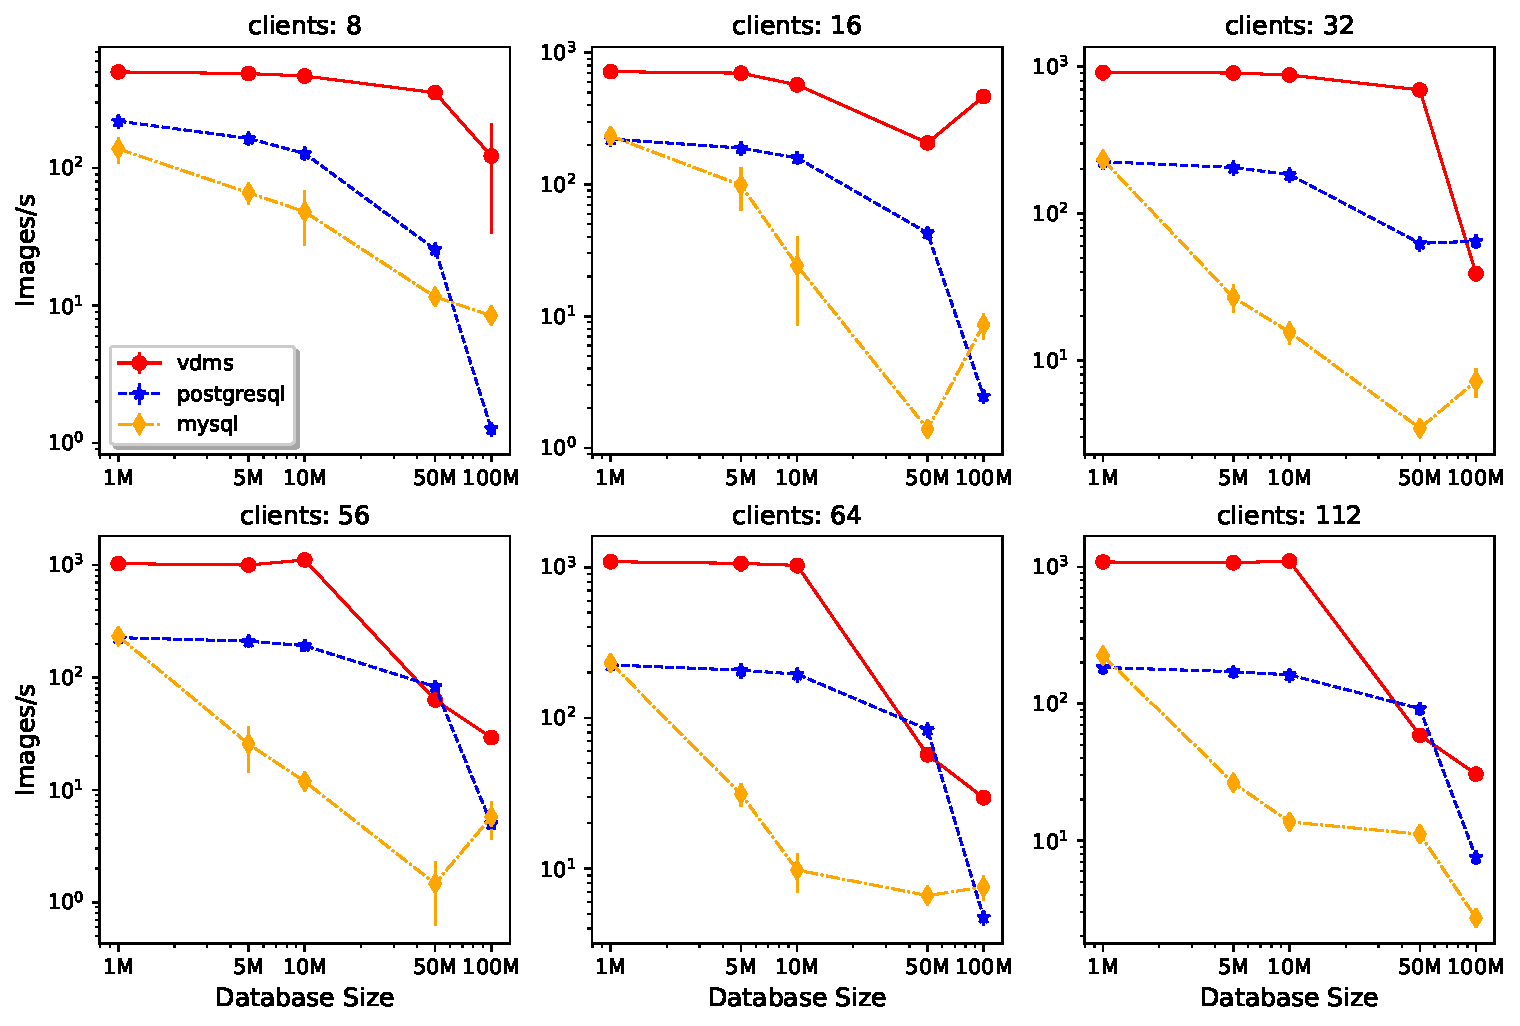
\includegraphics[width=\columnwidth]{figures/plot_q_2tag_resize_or_mosaic_results_throughput_threads}
\caption{Concurrency Analysis on \textit{q4} (\textit{2tag\_resize\_or}) from our use-case
described in the Experimental Setup Section.
The experiments show the throughput as images per second for
all systems (VDMS and two baselines) as the database size increases.}
\label{fig:concurrency_comparison_q4}
\end{figure}

In the case of \textit{q4} and \textit{q6}, we see the performance for \textit{mysql}
degrades up to 64 concurrent clients, then there's an improvement with 112 concurrent clients.
To further evaluate the concurrency of these queries with an OR operation, we continue by
looking at Figure~\ref{fig:concurrency_comparison_q4}. This figure illustrates a concurrency analysis for
\textit{q4} (\textit{2tag\_resize\_or}) which shows the images per second
delivered by each system as the database size grows (x-axis). We show different number
of concurrent clients in different figures for readability reasons.  For this query,
VDMS delivers higher throughput for databases 1M through 10M for all concurrent clients.
As the number of clients and the size of database grows, the performance for this query
drops and the performance of \textit{postgresql} becomes more comparable to VDMS. Lets look at the
case with 32 concurrent clients.
In this case, the throughput of VDMS drops drastically with
the 100M database and \textit{postgresql} outperforms by a small margin.
As the clients increase, we see this trade-off occurs with the 50M database
instead of 100M while in the 100M database, VDMS outperforms both baselines.
In this case, the throughput of \textit{postgresql} drastically degrades
for the 100M database and the performance of the baseline systems are more comparable.

When considering Figure~\ref{fig:concurrency_comparison_q2}
through Figure~\ref{fig:concurrency_comparison_q4},
there are many reasons why we generally see performance improvement, the main being
that the entire operation (metadata query, image fetching and resizing) happens
on the server side in the case of VDMS, within a single message
exchange between the client and the server.
Many of the inefficiencies that come with combining tools that were designed
without visual data in mind simply disappear when building a tool that treats
visual entities as first class citizens, as it is the case of VDMS.
Another reason, which is quantifiable in the figures, is that
VDMS sends resized (smaller) versions to the client instead of the full image
to be resized on the client side (as is the case in the baselines).
This is in contrast with the baseline implementations,
where 2 rounds of blocking back-and-forth communication with the server is needed,
as depicted in Figure~\ref{fig:systems}.
Note that one could argue that the opposite will happen
when the resize operation retrieves a an up-sampled (larger) version of the image
instead of a down-sampled (smaller) one.
In practice, retrieving an up-sampled version is not a common use case,
given that up-sampling the image does not add any extra information that can help,
for instance, improve the accuracy of a ML model.
The case of down-sampling the original image is much more common and is the common
practice when it comes to image processing through CNNs \cite{cnn,resnet}.

%% ========= Concurrency Comparison Analysis - END


%% ========= Queries Analysis

\subsubsection{Scalability Analysis}

% \begin{figure}[ht]
% % WAS: begin{figure*}[ht]; textwidth
% 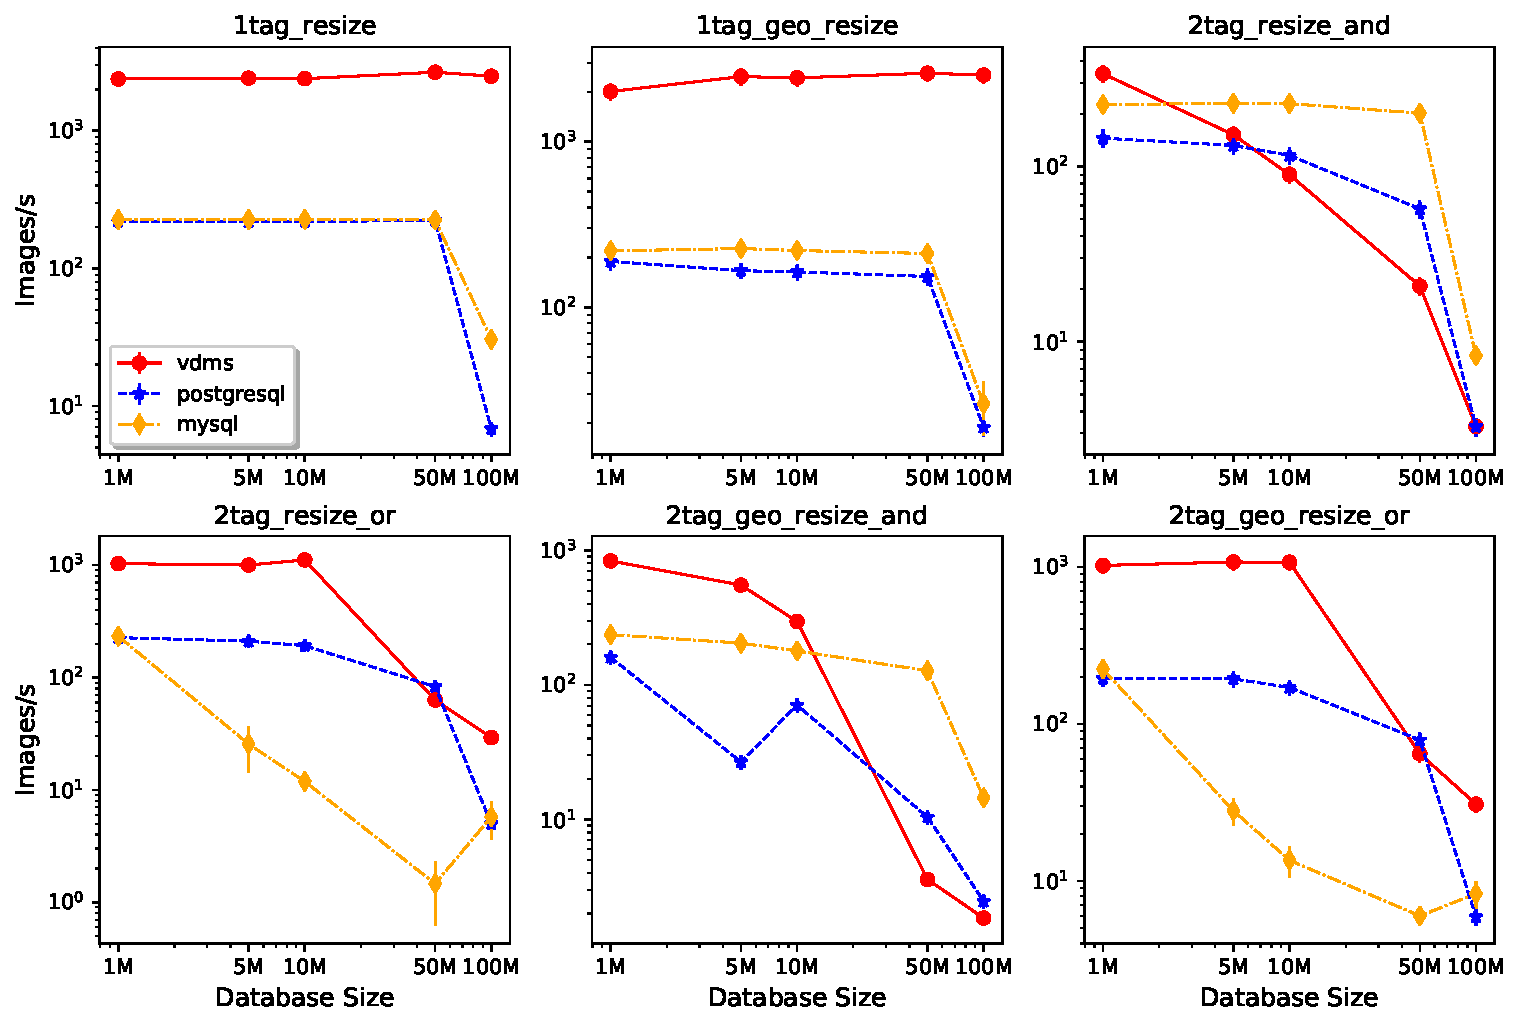
\includegraphics[width=\columnwidth]{figures/plot_th_56_mosaic_results_throughput}
% \caption{Throughput Analysis using all queries from our use-case
% described in the Experimental Setup Section.
% We show queries in different figures for readability reasons.
% The experiments show the performance of all systems (VDMS and the two baselines) as the
% database size increases.
% These queries were run using 56 simultaneous clients,
% and averaged out of 10 runs.}
% \label{fig:q_throughput_56}
% \end{figure}

The next step in our analysis involves looking more deeply at how
the performance scales with the number of elements in the database.
Figure~\ref{fig:q_throughput_56} shows the evaluation of the
queries we analysed for our use case.
Each figure shows the throughput when retrieving images,
plus operations applied to images when applicable.
The experiments show the performance of all systems (VDMS and two baselines) as the
database size increases in terms of number of images.
These queries were run using 56 simultaneous clients,
and averaged over 10 runs.
To analyze these plots, one needs to compare the full-line (VDMS) versus the
dotted-lines (two baselines), each plot representing a different query.

For \textit{q1} and \textit{q2}, we can appreciate higher performance being delivered by
VDMS when compared to the baselines, and how this improvement is maintained
as the size of the database increase while,
on the other hand, the baseline implementations have a drop in performance
for the 100M database.
For \textit{q3}, we see that VDMS performs best when the database size
is small (1M images), but as the database size increases,
the performance degrades as well.
For this query, \textit{mysql} (and in some cases \textit{postgresql}) outperforms VDMS
for databases larger than 1M.
This also occurs for \textit{q5} but only for databases larger than 10M.
This is entirely attributed to the 2-round process needed for this query,
as we explained before which is more visible in the larger databases.
It is interesting to note that adding filtering by geo-location
(\textit{q5}) decreases the performance as the database sizes scales.
The behavior is different in the case of \textit{q6},
which also filters by geo-location.
This is attributed to the fact that OR queries involves processing
larger results, and thus does not benefit from the filtering
which is evident when compared to \textit{q4}.

\begin{figure}[ht!]
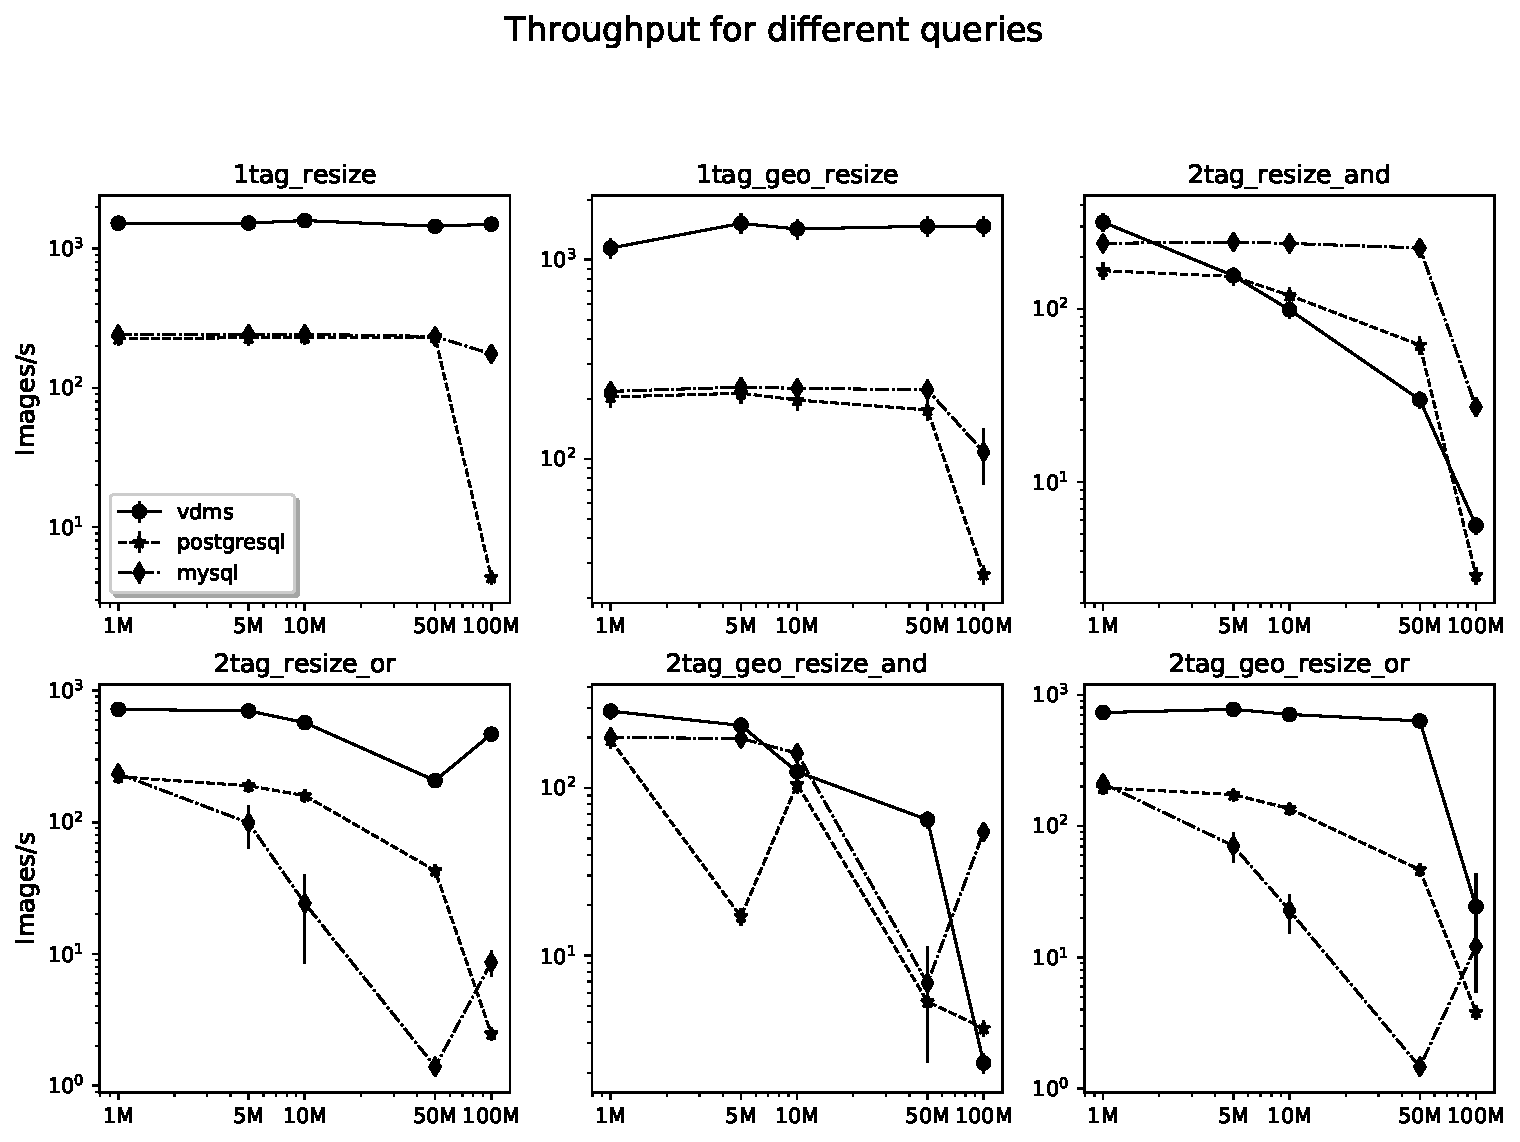
\includegraphics[width=\columnwidth]{figures/plot_th_16_mosaic_results_throughput}
\caption{Throughput Analysis using all queries from our use-case
described in the Experimental Setup Section.
We show queries in different figures for readability reasons.
The experiments show the performance of all systems (VDMS and the two baselines) as the
database size increases.
These queries were run using 16 simultaneous clients, and averaged out of 10 runs.}
\label{fig:q_throughput_16}
\end{figure}

%% ========= Resize Comparison

\begin{figure}[h!]
% WAS: begin{figure*}[ht]; textwidth
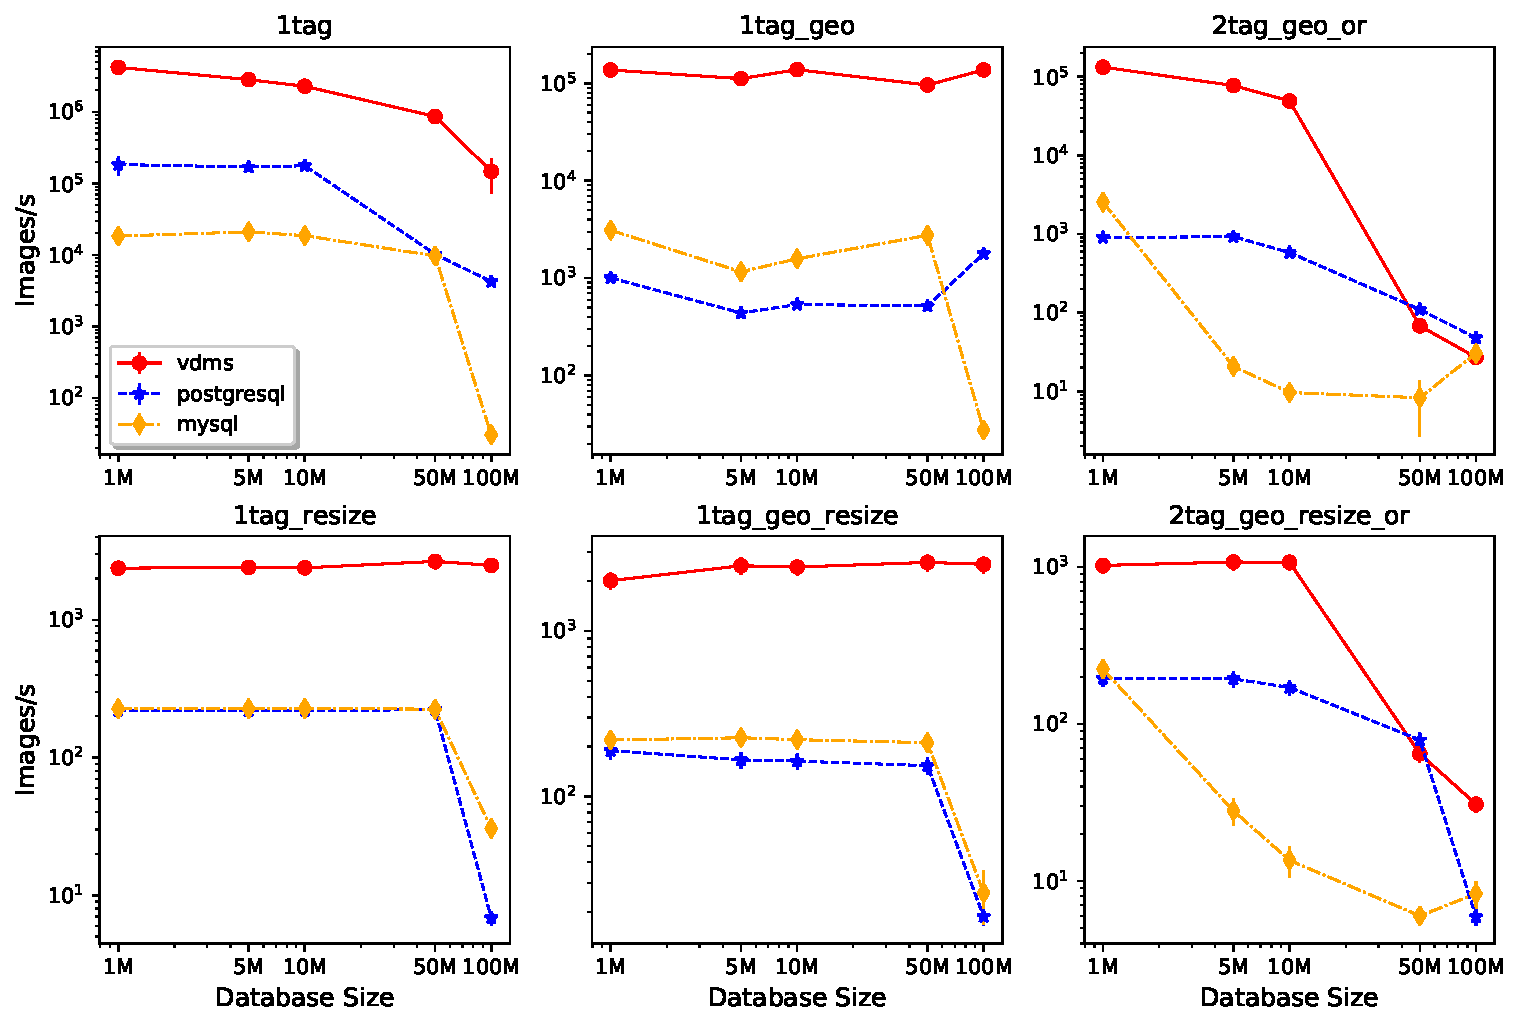
\includegraphics[width=\columnwidth]{figures/plot_th_56_mosaic_results_throughput_resize}
\caption{Throughput Analysis using a subset of the queries, with and without resize.}
\label{fig:q_throughput_56_resize}
\end{figure}

\begin{figure*}[ht!]
\centering
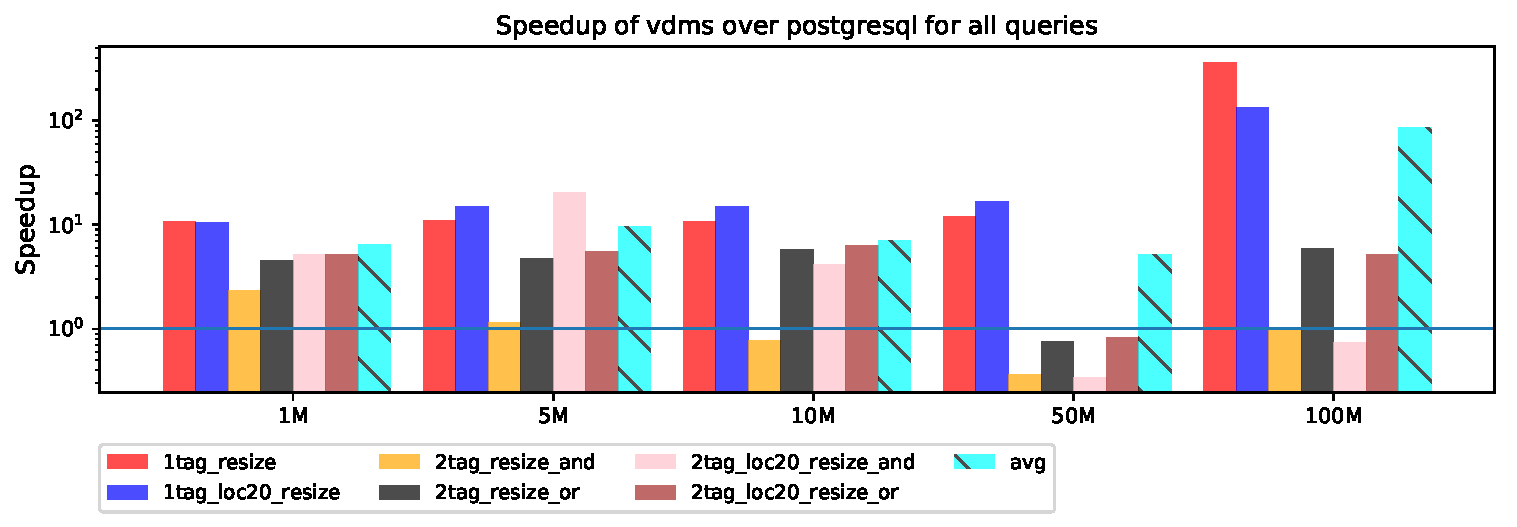
\includegraphics[width=\textwidth]{figures/plot_th_56_query_times_speedup_postgresql}
\caption{Summary of performance gains for all queries.
We see up to 364x speedup (\textit{q1}), and an average of about 85x.
More importantly, we see that the speedup grow as the database size increases,
showing that VDMS scales better than the PostgreSQL+Apache baseline.}
\label{fig:summary_postgresql}
\end{figure*}

From the first 2 queries, as well as \textit{q4} and
\textit{q6} (with exception to the 50M case),
we clearly see that VDMS outperforms the baseline systems
when retrieving visual data and applying operations.
This is one of the most important finding, as it validates the design principles
of VDMS, which aims to provide scalability and performance acceleration
at the type of queries that require visual data access and transformations.

% Figure~\ref{fig:q_throughput_16} shows the measured throughput,
% as images per second, delivered by each system for all queries and databases.
% In comparison to figure~\ref{fig:q_throughput_56},
% when using fewer concurrent clients (16),
% the throughput for VDMS for queries \textit{q4}, \textit{q5}, and \textit{q6}
% improved by a large margin for the 50M and 100M databases.
% In the case of \textit{q4} and \textit{q6},
% the throughput for 50M (and 100M for \textit{q4})
% increase by a large margin which outperforms both baselines while in
% Figure~\ref{fig:q_throughput_56} \textit{postgresql} slightly performed better than VDMS.
% In the case of \textit{q5}, all systems perform a little differently for databases
% larger than 5M.
% The gaps between the throughput of each system narrows at 10M.
% At a database size of 50M, the performance of the baselines drastically drop
% while the throughput of VDMS has a large improvement in comparison.


We designed VDMS with the idea in mind that pre-processing operations will be
commonly performed, as visual data is generally pre-processed before analytics
computation are performed on them.
Figure \ref{fig:q_throughput_56_resize} shows how the query throughput varies
when a pre-processing operations is applied (in this case, a resize operation).
The first thing to notice is that a resize operation is a significant part of
the overall operation (retrieval + preprocessing).
Doing a resize operation as part of the retrieval process
brings the throughput orders of magnitude down.
This is the case for both VDMS and the baseline.
Nonetheless, VDMS is orders of magnitude faster when retrieving images
both with and without resize operations.
An important thing to notice is that, even if a resized image is smaller,
and thus transfered faster between the server and the client,
transferring the image as is (without resize) is faster in this case.
This is a characteristic of the dataset, which has relatively small images
(the average image is about 150KB in size).
We have seen on other applications and datasets with higher resolution images
that transferring resized (or cropped) images is significantly faster than
transferring images as they are stored.
An interesting aspect to notice is that, when removing the resize operations,
differences between the 2 baseline systems become more noticeable.
For instance, for an image retrieval based on a single tag, we see how
\textit{postgresql} outperforms \textit{mysql}, but when adding geo-location
filtering, we see \textit{mysql} showing a small advantage.
When the resize operations is performed, both baselines do very similar
on 1tag based queries, and orders of magnitude worst than VDMS.
Note that in the baseline systems, the resize happens on the client side,
rather than on the server side.
This is the common case in most analytics applications, where pre-processing
operations happen on the client side (or when the analytics computation happens),
rather than near where the data is located, as it is the case with VDMS.
We kept both the server and client systems the same to avoid the computation
capabilities difference complicating our understanding of the results.


%% ========= Queries Analysis - END

%% ========= Summary Analysis


Finally, Figure~\ref{fig:summary_postgresql} summarizes the results
comparing VDMS and \textit{postgresql}.
In comparison to \textit{postgresql}, VDMS provides up to 364x speedup
(for the case of \textit{q1}),
and an average improvement in throughput of about 85x.
This is an impressive improvement over the two baseline systems.
More importantly, we see that the speedup increases as the database size grows,
showing that VDMS scales better than the baseline systems.
We also see how \textit{q3} and \textit{q5} have poor performances and scalability
when compared to the baselines as the database size grows, except in the
case of the largest database (100M), where the baselines performed very poorly.
This evaluation served the
purpose of understanding the importance of VDMS server side operators
that enable more complex queries for our use cases.
The team will address the missing implementation as part of future work.
Most of the performance improvements can be attributed to the design
principles of VDMS, which aims to eliminate the need of combining and
re-purposing systems that were designed to handle types of date other than visual.
VDMS, by design, eliminates most of the inefficiencies that result
from a forced integration of components designed for a
different range of applications.

Because of space constraints, we are only showing a subset of our evaluation.
More details about our comprehensive evaluation are available
\footnote{https://github.com/luisremis/visual\_storm/tree/master/yfcc100m/python/eval/results}.
% TODO. Upload the final version of the plots once we are sure we are not making
% more modifications.

%% ========= Summary Analysis - END
